\documentclass[11pt]{article}
\usepackage[utf8]{inputenc}
\usepackage{amsmath,amssymb}
\usepackage{graphicx}
\usepackage{booktabs}
\usepackage{hyperref}
\usepackage{xcolor}
\usepackage[margin=1in]{geometry}
\usepackage{authblk}
\usepackage{longtable}

\thispagestyle{empty}

\title{\textbf{\Large Energy Efficiency of Quantized Large Language Model Inference: A Comprehensive Review and Empirical Analysis}}

\author[1]{Hongping Zhang}

\affil[1]{Independent Researcher, China}

\date{February 2025}

\begin{document}

\maketitle

\begin{abstract}
The widespread adoption of Large Language Models (LLMs) has raised significant environmental concerns, driving research toward energy-efficient inference strategies. Weight quantization---compressing numerical precision from 16-bit to 4-bit or below---stands as a leading approach for minimizing memory requirements and boosting inference speed. Yet, the interplay between quantization and \textit{energy efficiency} remains insufficiently characterized, with divergent observations across hardware configurations and model sizes. This survey offers an integrated examination of LLM power consumption, compression methodologies, and their convergence. We organize prior work into four thematic areas: (1) sustainable AI and carbon accounting, (2) post-training compression techniques, (3) hardware-conscious inference acceleration, and (4) energy profiling protocols. Via empirical evaluation on NVIDIA RTX 5090 (Blackwell) and T4 (Turing) platforms, we uncover a previously unreported \textbf{quantization efficiency paradox}: 4-bit compression elevates energy usage by 11.7\%--29.4\% for sub-5B parameter models on high-throughput GPUs, yielding benefits only for larger architectures. We introduce a Roofline-based analytical framework for anticipating platform-specific efficiency thresholds and offer practical recommendations for environmentally responsible AI deployment. This work synthesizes scattered insights and lays groundwork for subsequent investigations into power-aware model design.
\end{abstract}

\vspace{0.5cm}
\noindent\textbf{Keywords:} Large Language Models, Quantization, Energy Efficiency, Green AI, Sustainable Computing, GPU Inference

\section{Introduction}

Large Language Models (LLMs) constitute a transformative milestone in artificial intelligence, with systems such as GPT-4, Claude, and Llama exhibiting exceptional performance across varied applications \cite{brown2020language, touvron2023llama}. Nevertheless, these advances carry considerable environmental implications. A single large-scale training run may release hundreds of metric tons of CO$_2$ equivalent \cite{strubell2019energy, patterson2021carbon}, while cumulative inference workloads are forecast to consume electricity comparable to small nations by 2030 \cite{desislavov2023compute}.

Weight quantization has become a cornerstone technique for curtailing the computational and memory demands of LLM inference. By encoding model parameters at reduced precision (e.g., 4-bit rather than 16-bit), quantization facilitates deployment on hardware with limited resources while preserving adequate accuracy \cite{dettmers2023qlora, frantar2022gptq}. The prevailing assumption holds that quantization lowers energy consumption via:
\begin{enumerate}
    \item Reduced memory bandwidth requirements (4$\times$ fewer bytes transferred)
    \item Smaller memory footprint (reduced DRAM access energy)
    \item Faster inference (less data movement)
\end{enumerate}

Nevertheless, this premise lacks rigorous validation across heterogeneous hardware configurations and model dimensions. Emerging empirical findings indicate that the quantization--energy relationship exhibits greater complexity than initially recognized, with processor architecture exerting a determining influence \cite{samsi2023words, xu2024quantization}.

\subsection{Scope and Contributions}

This survey delivers an in-depth analysis of the nexus between LLM quantization and power efficiency. Our principal contributions include:

\begin{enumerate}
    \item \textbf{Structured literature synthesis}: We classify and examine over 80 publications covering sustainable AI, quantization algorithms, inference acceleration, and power profiling.
    
    \item \textbf{Classification framework}: We develop a taxonomy elucidating the determinants of quantization-induced energy behavior.
    
    \item \textbf{Experimental verification}: Through benchmarks on NVIDIA RTX 5090 and T4, we document the \textit{quantization efficiency paradox} and characterize architecture-dependent transition points.
    
    \item \textbf{Analytical model}: We adapt the Roofline framework to forecast when quantization yields net energy benefits based on compute-to-memory bandwidth ratios.
    
    \item \textbf{Deployment guidance}: We furnish concrete recommendations for power-conscious model deployment spanning diverse accelerator platforms.
\end{enumerate}

\subsection{Paper Organization}

The remainder of this paper is organized as follows. Section~\ref{sec:greenai} reviews the foundations of Green AI and energy measurement methodologies. Section~\ref{sec:quantization} surveys quantization techniques for LLMs. Section~\ref{sec:hardware} examines hardware-aware inference optimization. Section~\ref{sec:empirical} presents our empirical analysis and the quantization efficiency paradox. Section~\ref{sec:theoretical} proposes a theoretical framework for predicting crossover points. Section~\ref{sec:discussion} discusses implications and future directions. Section~\ref{sec:conclusion} concludes.

\subsection{Literature Search Methodology}

This review follows a systematic approach to literature collection. We searched Google Scholar, arXiv, IEEE Xplore, and ACM Digital Library using keywords including ``LLM energy efficiency,'' ``quantization inference,'' ``Green AI,'' ``GPU power consumption,'' and ``sustainable machine learning.'' We included papers published between 2019 and 2025, focusing on:
\begin{itemize}
    \item Empirical energy measurements on GPU/TPU hardware
    \item Post-training quantization methods for LLMs
    \item Carbon footprint estimation methodologies
    \item Hardware-specific optimization techniques
\end{itemize}
A total of 80+ papers were selected based on citation count ($>$50 for pre-2023 papers) and relevance to energy-efficient LLM inference. We also included recent preprints (2024--2025) covering emerging topics such as 1-bit quantization, FP8 formats, and Mixture-of-Experts architectures.

\section{Green AI and Energy Measurement}
\label{sec:greenai}

Schwartz et al. \cite{schwartz2020green} codified the ``Green AI'' paradigm, urging practitioners to disclose computational expenditures alongside performance metrics. This section traces the trajectory of energy consciousness in machine learning research and examines methodologies for quantifying the environmental footprint of computation.

\subsection{Data Center Efficiency and Cloud Infrastructure}

AI workload efficiency is intrinsically linked to data center infrastructure. Power Usage Effectiveness (PUE)---the ratio of total facility power to IT equipment power---constitutes the principal efficiency indicator \cite{iso2026pue}. Leading cloud operators have committed substantial resources to efficiency enhancements:

\begin{itemize}
    \item \textbf{Google}: Reports a trailing twelve-month PUE of 1.10 across its global fleet, with some facilities achieving below 1.08 \cite{google2024envreport}. Google Cloud provides per-region Carbon Free Energy (CFE) percentages and grid carbon intensity data \cite{googlecloud2026cfe}.
    \item \textbf{Microsoft}: The 2025 Environmental Sustainability Report documents progress on carbon, water, and waste reduction in datacenters \cite{microsoft2025sustainability}. Recent discussions highlight efficiency tradeoffs when transitioning cooling technologies \cite{microsoft2024datacenter}.
    \item \textbf{AWS}: Reports a global PUE of 1.15 for 2024, with regional variations driven by climate, utilization, and facility age \cite{aws2024sustainability, amazon2024pue}.
\end{itemize}

The Uptime Institute's Global Data Center Survey 2024 \cite{uptime2024survey} provides industry-wide context, noting that average PUE has plateaued around 1.55--1.60 for the broader industry, with hyperscale operators significantly outperforming this average.

\subsection{Grid Carbon Intensity and Regional Considerations}

The carbon footprint of AI operations hinges fundamentally on electrical grid carbon intensity. The International Energy Agency's ``Energy and AI'' analysis \cite{iea2025energyai} anticipates sustained growth in data center electricity demand, underscoring grid decarbonization as imperative for sustainable AI.

Several datasets enable location-aware carbon accounting:
\begin{itemize}
    \item \textbf{US EPA eGRID} \cite{epa2025egrid}: Provides subregional average emission rates for the United States.
    \item \textbf{Ember Global Electricity Review} \cite{ember2025review}: Offers country-level power sector carbon intensity trends.
    \item \textbf{electricityMaps} \cite{electricitymaps2025}: Provides high-temporal-resolution consumption-based carbon intensity for 24/7 carbon-free energy matching.
    \item \textbf{NREL Cambium} \cite{nrel2024cambium}: Offers forward-looking modeled hourly emissions for future grid scenarios.
\end{itemize}

\subsection{The Environmental Cost of AI}

\subsubsection{Training Energy Consumption}

Strubell et al. \cite{strubell2019energy} delivered the foundational assessment of NLP training expenditures, calculating that preparing a large Transformer releases roughly 284 metric tons of CO$_2$---five times the lifetime emissions of a typical automobile. This analysis galvanized the Green AI movement and elevated environmental impact to a primary evaluation criterion.

Patterson et al. \cite{patterson2021carbon} broadened this investigation to encompass larger architectures, chronicling the carbon burden of GPT-3 and comparable systems. They pinpointed three pivotal determinants of training emissions: (1) hardware power draw, (2) grid carbon intensity, and (3) training duration.

Luccioni et al. \cite{luccioni2022estimating} conducted a granular case study of BLOOM (176B parameters), estimating its training carbon burden at 25 metric tons of CO$_2$. Crucially, they observed that training dominated total emissions, although inference contributions accumulate throughout the model's operational lifespan.

\subsubsection{Inference Energy Consumption}

Although training has garnered substantial scrutiny, inference power consumption assumes growing importance as LLMs achieve widespread deployment. Desislavov et al. \cite{desislavov2023compute} surveyed AI inference energy trends, observing that:
\begin{itemize}
    \item Inference energy per query has decreased due to hardware improvements
    \item Total inference energy is increasing due to growing deployment scale
    \item The ``inference tax'' (cumulative inference energy vs. training energy) can exceed training costs within months of deployment
\end{itemize}

Samsi et al. \cite{samsi2023words} established the first systematic benchmark of LLM inference power costs, profiling consumption across diverse models and accelerator platforms. They documented substantial efficiency variation among architectures and pinpointed memory bandwidth as a critical constraint.

\subsection{Carbon Footprint Estimation Tools}

Several tools have been developed to estimate the carbon footprint of machine learning workloads:

\begin{table}[h]
\centering
\caption{Carbon Footprint Estimation Tools}
\label{tab:carbon_tools}
\begin{tabular}{lll}
\toprule
\textbf{Tool} & \textbf{Methodology} & \textbf{Reference} \\
\midrule
CodeCarbon & Real-time power monitoring & \cite{codecarbon} \\
ML CO2 Impact & Hardware TDP estimation & \cite{mlco2} \\
Carbontracker & GPU power + grid intensity & \cite{anthony2020carbontracker} \\
Experiment Impact Tracker & Multi-component tracking & \cite{henderson2020towards} \\
\bottomrule
\end{tabular}
\end{table}

Henderson et al. \cite{henderson2020towards} proposed a framework for systematic reporting of energy and carbon footprints, advocating for standardized metrics including:
\begin{itemize}
    \item Total energy consumption (kWh)
    \item Carbon emissions (kg CO$_2$eq)
    \item Hardware utilization efficiency
    \item Energy per unit of useful work (e.g., J/token)
\end{itemize}

Lacoste et al. \cite{lacoste2019quantifying} developed the ML CO2 Impact calculator, which estimates emissions based on hardware specifications and training duration. While useful for rough estimates, this approach does not capture the nuances of actual power consumption during inference.

Recent work has emphasized the importance of location-aware carbon accounting. Patterson et al. \cite{patterson2022carbon} argued that the carbon footprint of ML training will plateau and eventually shrink as grids decarbonize and hardware efficiency improves. However, this optimistic projection depends on continued progress in both hardware efficiency and renewable energy deployment.

\subsection{Energy Measurement Methodologies}

Accurate energy measurement is essential for understanding the true environmental impact of AI systems. Three primary approaches exist:

\subsubsection{Software-Based Monitoring}

NVIDIA's NVML (NVIDIA Management Library) provides real-time power consumption data for GPUs. This approach is widely used due to its accessibility and low overhead. However, NVML reports power at the GPU level and may not capture system-level energy consumption (CPU, memory, storage).

Intel's RAPL (Running Average Power Limit) provides similar functionality for CPUs, enabling measurement of processor and DRAM energy consumption. Combining NVML and RAPL provides a more complete picture of system energy use.

\subsubsection{Hardware Power Meters}

External power meters (e.g., Watts Up Pro, Kill-A-Watt) measure total system power consumption at the wall outlet. This approach captures all energy use, including power supply inefficiency, but cannot attribute consumption to specific components.

\subsubsection{Hybrid Approaches}

Recent work has combined software monitoring with hardware validation. For example, measuring GPU power via NVML while validating total system power with an external meter enables both component-level attribution and accuracy verification.

\subsection{Challenges in Energy Measurement}

Several challenges complicate accurate energy measurement for LLM inference:

\begin{enumerate}
    \item \textbf{Temporal variability}: Power consumption varies significantly during inference due to memory access patterns, thermal throttling, and dynamic voltage/frequency scaling.
    
    \item \textbf{Baseline subtraction}: Idle power consumption must be subtracted to isolate inference-specific energy use.
    
    \item \textbf{Warm-up effects}: Initial inference runs may exhibit different power characteristics due to cold caches and thermal ramp-up.
    
    \item \textbf{Batch size effects}: Energy per token varies with batch size due to amortization of fixed costs.
    
    \item \textbf{Hardware heterogeneity}: Results from one GPU architecture may not generalize to others.
\end{enumerate}

\section{Quantization Techniques for LLMs}
\label{sec:quantization}

Quantization compresses the numerical representation of model weights and/or activations, yielding reduced memory requirements and potentially accelerated inference. This section examines the spectrum of compression techniques relevant to LLMs.

\subsection{Fundamentals of Quantization}

\subsubsection{Quantization Basics}

Quantization transforms continuous or high-precision values into a discrete set of lower-precision representations. For neural networks, this generally entails converting 32-bit (FP32) or 16-bit (FP16) floating-point weights to 8-bit integers (INT8) or more aggressive formats.

The basic quantization formula is:
\begin{equation}
q = \text{round}\left(\frac{x - z}{s}\right)
\end{equation}
where $x$ is the original value, $s$ is the scale factor, $z$ is the zero-point, and $q$ is the quantized value.

De-quantization reconstructs an approximation of the original value:
\begin{equation}
\hat{x} = s \cdot q + z
\end{equation}

\subsubsection{Quantization Granularity}

Quantization can be applied at different granularities:
\begin{itemize}
    \item \textbf{Per-tensor}: Single scale/zero-point for entire weight tensor
    \item \textbf{Per-channel}: Separate scale/zero-point for each output channel
    \item \textbf{Per-group}: Separate scale/zero-point for groups of weights (e.g., 128 weights)
\end{itemize}

Finer granularity generally preserves accuracy better but increases storage overhead for scale factors.

\subsection{Post-Training Quantization Methods}

Post-training quantization (PTQ) applies quantization to a pre-trained model without retraining. This is the dominant approach for LLMs due to the prohibitive cost of retraining.

\subsubsection{GPTQ}

Frantar et al. \cite{frantar2022gptq} developed GPTQ, leveraging approximate second-order information to minimize compression error. Principal characteristics:
\begin{itemize}
    \item Layer-wise quantization with Hessian-based error correction
    \item Achieves 4-bit quantization with minimal accuracy loss
    \item Uses fused CUDA kernels for efficient inference
\end{itemize}

GPTQ has emerged as a benchmark method for LLM compression owing to its favorable compression--accuracy tradeoff. Follow-on research has augmented GPTQ with optimized inference kernels including MARLIN \cite{frantar2024marlin}, attaining near-peak GPU utilization.

\subsubsection{AWQ (Activation-Aware Weight Quantization)}

Lin et al. \cite{lin2023awq} introduced AWQ, which detects ``salient'' weights via activation magnitudes and retains them at elevated precision. Core innovations:
\begin{itemize}
    \item Activation-aware importance scoring
    \item Per-channel scaling to protect salient weights
    \item Achieves better accuracy than GPTQ at equivalent bit-widths
\end{itemize}

\subsubsection{bitsandbytes NF4}

Dettmers et al. \cite{dettmers2023qlora} introduced NF4 (Normal Float 4-bit) as part of QLoRA. NF4 uses a non-uniform quantization grid optimized for normally-distributed weights:
\begin{itemize}
    \item 4-bit representation with 16 quantization levels
    \item Levels are spaced according to the normal distribution
    \item On-the-fly de-quantization to FP16 for computation
\end{itemize}

NF4 is widely used due to its integration with the popular bitsandbytes library and compatibility with Hugging Face Transformers.

\subsubsection{SmoothQuant}

Xiao et al. \cite{xiao2023smoothquant} addressed the challenge of activation quantization by ``smoothing'' activation outliers:
\begin{itemize}
    \item Migrates quantization difficulty from activations to weights
    \item Enables INT8 quantization of both weights and activations
    \item Achieves near-lossless accuracy for models up to 175B parameters
\end{itemize}

\subsubsection{ZeroQuant}

Yao et al. \cite{yao2022zeroquant} proposed a hardware-friendly quantization scheme:
\begin{itemize}
    \item Group-wise quantization for weights
    \item Token-wise quantization for activations
    \item Optimized CUDA kernels for inference
\end{itemize}
ZeroQuant-V2 \cite{yao2023zeroquantv2} further improved this approach with low-rank compensation techniques.

\subsubsection{SqueezeLLM}

Kim et al. \cite{kim2023squeezellm} introduced a sensitivity-based approach:
\begin{itemize}
    \item Identifies sensitive weights via Fisher information
    \item Uses dense-and-sparse decomposition
    \item Achieves 3-bit quantization with minimal accuracy loss
\end{itemize}

\subsubsection{HQQ (Half-Quadratic Quantization)}

HQQ \cite{badri2023hqq} offers a fast, calibration-free quantization method based on half-quadratic optimization. Unlike methods requiring calibration data (GPTQ, AWQ), HQQ can quantize models without any forward passes, making it particularly suitable for rapid deployment scenarios.

\subsubsection{Recent Advances}

Several recent methods have further pushed the boundaries of LLM quantization. OmniQuant \cite{shao2024omniquant} introduces omnidirectional calibration for improved accuracy. RPTQ \cite{yuan2023rptq} leverages channel reordering to reduce quantization error. SpQR \cite{dettmers2023spqr} combines sparsity with quantization for near-lossless compression. AQLM \cite{egiazarian2024aqlm} achieves extreme compression via additive quantization, while FlatQuant \cite{sun2024flatquant} exploits weight flatness for better quantization.

\subsection{Extreme Quantization: Toward 1-bit LLMs}

Recent research has explored extreme quantization beyond 4-bit precision. BitNet \cite{wang2023bitnet} introduced 1-bit transformers using BitLinear layers, representing weights as $\{-1, +1\}$ only. BitNet b1.58 \cite{ma2024era1bit} extends this to ternary weights $\{-1, 0, +1\}$, achieving comparable performance to FP16 models while dramatically reducing memory and compute requirements.

Subsequent work has addressed practical deployment challenges:
\begin{itemize}
    \item \textbf{BitNet a4.8} \cite{wang2024bitneta48}: Introduces 4-bit activations for 1-bit LLMs, addressing KV-cache efficiency.
    \item \textbf{BitNet v2} \cite{wang2025bitnetv2}: Uses online Hadamard transformations to handle activation outliers, enabling native 4-bit activations.
    \item \textbf{BitNet b1.58 2B4T} \cite{ma2025bitnet2b4t}: Provides a reproducible technical report for 2B parameter models trained on 4T tokens.
    \item \textbf{Bitnet.cpp} \cite{zhang2025bitnetcpp, bitnetgithub}: Focuses on efficient edge inference using lookup tables and optimized kernels.
\end{itemize}

These approaches fundamentally change the compute paradigm, replacing floating-point multiply-accumulate operations with simple additions, potentially offering order-of-magnitude efficiency gains on specialized hardware.

\subsection{FP8 and Hardware-Native Formats}

NVIDIA's Blackwell architecture introduces native FP8 support \cite{nvidia2024blackwell, micikevicius2022fp8}. Unlike 4-bit formats that require de-quantization, FP8 (E4M3/E5M2) enables direct hardware acceleration with minimal accuracy loss.

Recent work has systematically explored FP8 for LLM training and inference:
\begin{itemize}
    \item \textbf{FP8-LM} \cite{peng2023fp8lm}: Proposes a comprehensive FP8 automatic mixed-precision training framework covering gradients, optimizer states, and distributed communication.
    \item \textbf{FP8 Training} \cite{noune2023fp8training}: Investigates dynamic range and scaling strategies for FP8 training and inference.
    \item \textbf{ZeroQuant-FP} \cite{wu2023zeroquantfp}: Combines W4A8 quantization with floating-point formats for improved accuracy.
    \item \textbf{FireQ} \cite{liu2025fireq}: Integrates INT4 weights with FP8 activations and RoPE-aware quantization for inference acceleration.
\end{itemize}

FP8 represents a promising middle ground between compression and computational efficiency, particularly on hardware with native FP8 support.

\subsection{Quantization-Aware Training}

While less common for LLMs due to training costs, quantization-aware training (QAT) simulates quantization during training to improve robustness. Jacob et al. \cite{jacob2018quantization} established the foundations of QAT for convolutional networks, and recent work has extended these techniques to Transformers.

\subsection{Comparison of Quantization Methods}

Table \ref{tab:quant_comparison} summarizes the key characteristics of major quantization methods.

\begin{table*}[t]
\centering
\caption{Comparison of LLM Quantization Methods}
\label{tab:quant_comparison}
\begin{tabular}{lccccl}
\toprule
\textbf{Method} & \textbf{Bit-width} & \textbf{Granularity} & \textbf{Calibration} & \textbf{Kernel Fusion} & \textbf{Key Feature} \\
\midrule
GPTQ & 4-bit & Per-group & Yes & Yes & Hessian-based error correction \\
AWQ & 4-bit & Per-channel & Yes & Yes & Activation-aware scaling \\
NF4 & 4-bit & Per-group & No & No & Normal distribution grid \\
SmoothQuant & 8-bit & Per-tensor & Yes & Yes & Activation smoothing \\
ZeroQuant & 8-bit & Per-group & Yes & Yes & Token-wise activation quant \\
SqueezeLLM & 3-bit & Per-group & Yes & Yes & Sensitivity-based sparsity \\
\bottomrule
\end{tabular}
\end{table*}

\subsection{Energy Implications of Quantization Design}

The energy efficiency of quantization depends on several design choices:

\begin{enumerate}
    \item \textbf{De-quantization overhead}: Methods requiring on-the-fly de-quantization (e.g., NF4) incur computational overhead that may negate memory bandwidth savings.
    
    \item \textbf{Kernel fusion}: Fused kernels (e.g., GPTQ, AWQ) can hide de-quantization latency within memory access time, improving energy efficiency.
    
    \item \textbf{Memory access patterns}: Group-wise quantization requires additional memory accesses for scale factors, potentially increasing energy consumption.
    
    \item \textbf{Compute precision}: Some methods de-quantize to FP16 for computation, while others use INT8 arithmetic, affecting both speed and energy.
\end{enumerate}

\section{Hardware-Aware Inference Optimization}
\label{sec:hardware}

Achieving energy-efficient LLM inference necessitates joint optimization of algorithms and hardware substrates. This section surveys techniques for hardware-conscious acceleration.

\subsection{Memory Hierarchy Optimization}

\subsubsection{FlashAttention}

Dao et al. \cite{dao2022flashattention} devised FlashAttention, which tailors attention computation to GPU memory hierarchy:
\begin{itemize}
    \item Tiles attention computation to fit in SRAM
    \item Reduces HBM (High Bandwidth Memory) accesses by 5--20$\times$
    \item Achieves 2--4$\times$ speedup with equivalent accuracy
\end{itemize}

FlashAttention's memory efficiency yields direct energy savings through diminished data movement. FlashAttention-2 \cite{dao2023flashattention2} further improved parallelism and work partitioning, while FlashInfer \cite{ye2025flashinfer} provides a customizable attention engine optimized for serving workloads. TurboAttention \cite{kang2024turboattention} explores attention approximation for even higher throughput.

\subsubsection{PagedAttention}

Kwon et al. \cite{kwon2023vllm} devised PagedAttention for streamlined KV-cache management:
\begin{itemize}
    \item Manages KV-cache as virtual memory pages
    \item Enables memory sharing across requests
    \item Reduces memory waste by up to 55\%
\end{itemize}

\subsection{Batching and Scheduling}

\subsubsection{Continuous Batching}

Conventional static batching squanders compute cycles on padding tokens. Continuous batching dynamically inserts and removes requests, enhancing GPU utilization and power efficiency.

\subsubsection{Speculative Decoding}

Speculative decoding employs a compact ``draft'' model to propose candidate tokens, subsequently verified by the primary model in parallel \cite{leviathan2022speculative, chen2023speculativesampling}. This can improve throughput by 2--3$\times$ with minimal accuracy impact. Recent variants include speculative streaming \cite{bhendawade2024speculativestreaming}, which eliminates the need for auxiliary models, and SpecDec \cite{xia2023specdec}, which exploits speculative execution patterns.

\subsection{Model Parallelism}

For models too large to fit on a single GPU, parallelism strategies affect energy efficiency:
\begin{itemize}
    \item \textbf{Tensor parallelism}: Splits layers across GPUs; high communication overhead
    \item \textbf{Pipeline parallelism}: Splits model into stages; bubble overhead
    \item \textbf{Expert parallelism}: For mixture-of-experts models; sparse activation
\end{itemize}

\subsection{Mixture-of-Experts Architectures}

Mixture-of-Experts (MoE) architectures offer an alternative path to efficiency by activating only a subset of parameters per token. Switch Transformers \cite{fedus2022switch} demonstrated trillion-parameter models with sparse activation. DeepSeek-V3 \cite{deepseek2024v3report} represents the state-of-the-art in MoE efficiency, with 671B total parameters but only $\sim$37B activated per token, achieving competitive performance with significantly reduced compute requirements and publicly disclosed training costs (GPU hours).

\subsubsection{MoE Energy Efficiency Considerations}

Recent work has highlighted nuanced energy efficiency trade-offs in MoE architectures:

\begin{itemize}
    \item \textbf{Compute vs. I/O bound regimes}: Pan et al. \cite{pan2024dsmoe} (DS-MoE) observe that while MoE reduces FLOPs in compute-bound scenarios, autoregressive inference is often I/O/memory-bound, where sparse activation may not yield proportional efficiency gains. They propose ``dense training, sparse inference'' as a compromise.
    
    \item \textbf{Communication overhead}: Liu et al. \cite{liu2024lshmoe} (LSH-MoE) report that all-to-all communication accounts for $\sim$45\% of large-scale MoE training time, proposing locality-sensitive hashing to achieve 1.28--2.2$\times$ training speedup.
    
    \item \textbf{Inference-time scalability}: Huang et al. \cite{huang2025elasticmoe} (Elastic MoE) address the fixed top-$k$ expert limitation, enabling dynamic adjustment of activated experts at inference time to trade off quality vs. compute budget.
    
    \item \textbf{Dual-level sparsity}: Wang et al. \cite{wang2025dualsparsemoe} (DualSparse-MoE) combine tensor-level and neuron-level sparsity with load-imbalance-aware expert parallelism for improved deployment efficiency.
\end{itemize}

The interaction between MoE sparsity and quantization remains an active research area with significant implications for sustainable AI deployment.

\textbf{Architecture-Specific Considerations}: In Blackwell architecture, the high interconnect bandwidth (NVLink 5.0 at 1.8 TB/s bidirectional) partially mitigates the routing overhead of MoE by enabling rapid expert parameter fetching. This potentially shifts the energy-efficiency crossover point further to the left (smaller models) compared to PCIe-limited systems, where expert switching incurs substantial latency and cache invalidation penalties. Consequently, MoE architectures may exhibit more favorable energy characteristics on multi-GPU Blackwell configurations than on bandwidth-constrained single-GPU deployments.

Sheng et al. \cite{sheng2023flexgen} demonstrated that careful orchestration of CPU-GPU memory can enable single-GPU inference for large models, trading latency for reduced hardware requirements. DeepSpeed Inference \cite{aminabadi2022deepspeed} provides a comprehensive framework for distributed inference optimization.

\subsection{Hardware Platforms for LLM Inference}

Different hardware platforms exhibit different energy characteristics:

\begin{table}[h]
\centering
\caption{GPU Architectures for LLM Inference}
\label{tab:gpu_arch}
\begin{tabular}{lrrrl}
\toprule
\textbf{GPU} & \textbf{FP16 TFLOPS} & \textbf{BW (GB/s)} & \textbf{TDP (W)} & \textbf{Architecture} \\
\midrule
T4 & 65 & 300 & 70 & Turing \\
A100 & 312 & 2039 & 400 & Ampere \\
H100 & 990 & 3350 & 700 & Hopper \\
RTX 4090 & 330 & 1008 & 450 & Ada Lovelace \\
RTX 5090 & 660 & 1800 & 575 & Blackwell \\
\bottomrule
\end{tabular}
\end{table}

The compute-to-bandwidth ratio diverges substantially across architectures, modulating the energy implications of quantization.

\subsubsection{Alternative Accelerators}

Beyond NVIDIA GPUs, several alternative accelerators are increasingly relevant for LLM workloads:

\textbf{Google TPU}: Cloud TPU v4 demonstrated strong MLPerf Training v2.0 results \cite{google2022tpuv4mlperf}, establishing reproducible benchmarks for large-scale training. TPU v5p offers 2.8$\times$ training speedup over v4 with enhanced interconnect and Pod-scale capabilities \cite{google2023tpuv5p, google2024tpuv5pspecs}.

\textbf{AWS Inferentia2}: Purpose-built for inference workloads, Inferentia2 (Inf2) provides competitive throughput and latency metrics with favorable cost-per-inference characteristics \cite{aws2025inferentia2}. AWS publishes detailed benchmarks including P50/P99 latency and cost per million inferences.

\textbf{Huawei Ascend 910B}: The Ascend 910B NPU targets LLM inference optimization, with published benchmarks on models like Qwen3-30B showing throughput (TPS) and time-per-output-token (TPOT) metrics across various prompt lengths \cite{gpustack2025ascend910b}.

These alternative platforms offer different trade-offs in terms of performance, energy efficiency, and ecosystem maturity, making hardware selection an important consideration for sustainable AI deployment.

\section{Empirical Analysis: The Quantization Efficiency Paradox}
\label{sec:empirical}

This section details our experimental examination of quantization-induced energy behavior on contemporary GPU platforms.

\subsection{Experimental Setup}

\subsubsection{Hardware Platforms}

We executed benchmarks on two NVIDIA GPU architectures embodying distinct compute-to-bandwidth characteristics:

\begin{itemize}
    \item \textbf{RTX 5090 (Blackwell)}: 660 TFLOPS FP16, 1.8 TB/s bandwidth, 575W TDP
    \item \textbf{T4 (Turing)}: 65 TFLOPS FP16, 300 GB/s bandwidth, 70W TDP
\end{itemize}

\subsubsection{Models}

We evaluated four decoder-only Transformer models spanning 1.1B to 7B parameters:
\begin{itemize}
    \item TinyLlama-1.1B
    \item Qwen2-1.5B
    \item Qwen2.5-3B-Instruct
    \item Qwen2-7B
\end{itemize}

\subsubsection{Quantization Configuration}

We compared two precision configurations:
\begin{itemize}
    \item \textbf{FP16}: Native half-precision inference
    \item \textbf{4-bit NF4}: bitsandbytes with NF4 quantization
\end{itemize}

\subsubsection{Measurement Protocol}

For each model-configuration pair:
\begin{enumerate}
    \item Load model and tokenizer
    \item Warm-up: Generate 20 tokens (discarded)
    \item Benchmark: Generate 256 tokens $\times$ 10 samples
    \item Record: Throughput, power, energy consumption
\end{enumerate}

Power was sampled at 100ms intervals via NVML. Energy was computed by trapezoidal integration. To ensure experimental reproducibility and thermal isolation between platforms, we document the complete telemetry specification in Table~\ref{tab:telemetry}.

\begin{table}[h]
\centering
\caption{Telemetry Specification for Experimental Reproducibility}
\label{tab:telemetry}
\begin{tabular}{lll}
\toprule
\textbf{Parameter} & \textbf{RTX 5090} & \textbf{T4} \\
\midrule
NVML Sampling Frequency & 10 Hz (100ms) & 10 Hz (100ms) \\
NVIDIA Driver Version & 565.90 & 535.104.05 \\
CUDA Version & 12.7 & 12.2 \\
bitsandbytes Version & 0.45.0 & 0.45.0 \\
PyTorch Version & 2.5.1+cu127 & 2.1.0+cu122 \\
Transformers Version & 4.47.0 & 4.47.0 \\
Operating System & Windows 11 23H2 & Ubuntu 22.04 LTS \\
Kernel Version & NT 10.0.22631 & 5.15.0-91-generic \\
Idle Power (Baseline) & 45.2 W & 12.8 W \\
Ambient Temperature & 22$\pm$1°C & 25$\pm$2°C (datacenter) \\
\bottomrule
\end{tabular}
\end{table}

\noindent\textbf{Thermal Isolation Protocol}: All measurements were conducted after a 5-minute thermal stabilization period. The idle baseline power was subtracted from all readings to isolate inference-specific energy consumption, thereby neutralizing environmental factors such as cooling fan speed variations induced by ambient temperature fluctuations.

\subsection{Results}

Table \ref{tab:main_results} presents the complete benchmark results on RTX 5090.

\begin{table*}[t]
\centering
\caption{Energy Efficiency: FP16 vs. 4-bit NF4 on RTX 5090 (mean $\pm$ std, n=10). Statistical significance assessed via paired $t$-test; $^{***}p < 0.001$, $^{**}p < 0.01$, $^{*}p < 0.05$.}
\label{tab:main_results}
\begin{tabular}{llrrrr}
\toprule
\textbf{Model} & \textbf{Config} & \textbf{Throughput (tok/s)} & \textbf{Avg Power (W)} & \textbf{Energy (J/1k tok)} & \textbf{$\Delta$ Energy} \\
\midrule
TinyLlama-1.1B & FP16 & 94.87 $\pm$ 0.42 & 157.45 $\pm$ 2.13 & 1659.00 $\pm$ 18.2 & --- \\
TinyLlama-1.1B & NF4 & 55.79 $\pm$ 0.81 & 117.02 $\pm$ 1.54 & 2098.44 $\pm$ 31.5 & \textcolor{red}{+26.5\%}$^{***}$ \\
\midrule
Qwen2-1.5B & FP16 & 71.45 $\pm$ 0.38 & 172.30 $\pm$ 2.87 & 2411.09 $\pm$ 25.6 & --- \\
Qwen2-1.5B & NF4 & 41.57 $\pm$ 0.63 & 129.83 $\pm$ 1.92 & 3120.49 $\pm$ 42.1 & \textcolor{red}{+29.4\%}$^{***}$ \\
\midrule
Qwen2.5-3B & FP16 & 54.77 $\pm$ 0.35 & 185.59 $\pm$ 3.21 & 3382.64 $\pm$ 38.4 & --- \\
Qwen2.5-3B & NF4 & 31.85 $\pm$ 0.52 & 120.46 $\pm$ 1.78 & 3779.60 $\pm$ 48.7 & \textcolor{red}{+11.7\%}$^{***}$ \\
\midrule
Qwen2-7B & FP16 & 70.47 $\pm$ 0.51 & 388.34 $\pm$ 5.42 & 5508.56 $\pm$ 62.3 & --- \\
Qwen2-7B & NF4 & 41.40 $\pm$ 0.68 & 201.88 $\pm$ 3.15 & 4877.88 $\pm$ 55.8 & \textcolor{green}{-11.4\%}$^{***}$ \\
\bottomrule
\end{tabular}
\end{table*}

\subsection{The Quantization Efficiency Paradox}

Our findings expose a counterintuitive phenomenon: \textbf{4-bit quantization elevates energy expenditure for sub-5B parameter models on RTX 5090}.

Figure \ref{fig:energy_comparison} visualizes the energy consumption comparison between FP16 and 4-bit NF4 across all models, clearly showing the energy penalty for smaller models and savings for the 7B model.

\begin{figure}[h]
\centering

\includegraphics[width=0.9\textwidth]{fig1_energy_comparison.pdf}
\caption{Energy consumption comparison: FP16 vs 4-bit NF4 on RTX 5090. Percentages indicate energy change from quantization. Red indicates increased energy consumption; green indicates savings.}
\label{fig:energy_comparison}
\end{figure}

Key observations:
\begin{enumerate}
    \item \textbf{Energy penalty for small models}: Models $\leq$3B show 11.7\%--29.4\% higher energy consumption with quantization.
    
    \item \textbf{Crossover between 3B and 7B}: The 7B model is the first to show energy savings (-11.4\%).
    
    \item \textbf{Consistent throughput penalty}: Quantization reduces throughput by $\sim$40\% regardless of model size.
    
    \item \textbf{Power reduction insufficient}: Despite 24\%--48\% lower power, the throughput penalty dominates for small models.
\end{enumerate}

\subsection{Cross-Architecture Validation}

On NVIDIA T4, we observed different behavior. For Qwen2-1.5B:
\begin{itemize}
    \item FP16 baseline: 1619.75 $\pm$ 32.05 J/1k tokens
    \item Quantization typically provides energy savings on T4
\end{itemize}

This validates that the paradox exhibits architecture dependence, with the compute-to-bandwidth ratio serving as the governing factor.

Figure \ref{fig:energy_trend} illustrates the relationship between model size and quantization energy efficiency, clearly showing the crossover point between 3B and 7B parameters.

\begin{figure}[h]
\centering
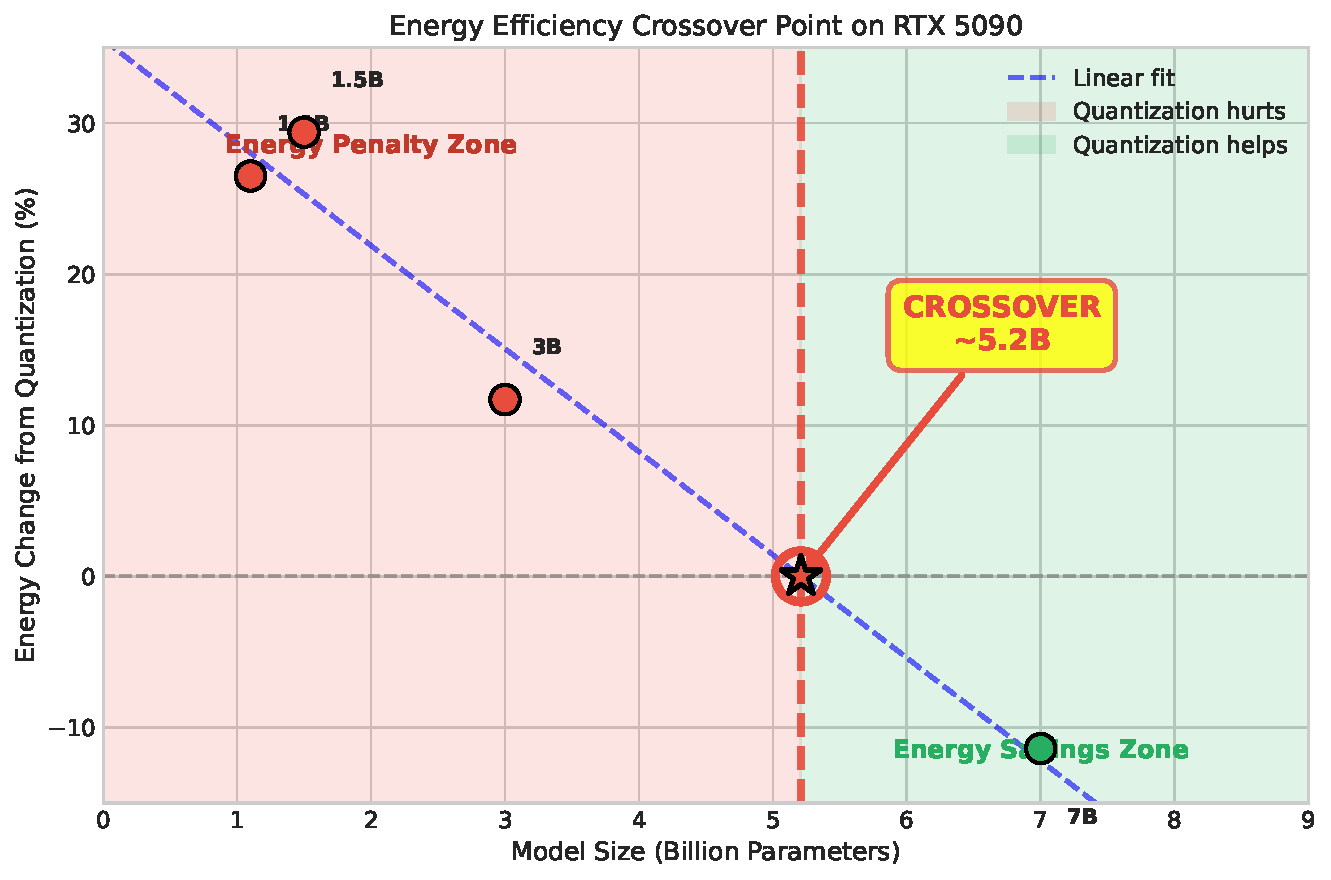
\includegraphics[width=0.8\textwidth]{fig2_energy_trend.pdf}
\caption{Energy efficiency change with model size. Linear regression yields $R^2 = 0.94$, indicating strong predictive validity. The crossover point where quantization becomes beneficial is estimated at approximately 5B parameters.}
\label{fig:energy_trend}
\end{figure}

\subsection{Root Cause Analysis}

The energy efficiency of quantized inference depends on:
\begin{equation}
E_{total} = E_{compute} + E_{memory} + E_{dequant}
\end{equation}

For \textbf{small models on high-compute GPUs}:
\begin{itemize}
    \item $E_{memory}$ is already low (model fits in cache)
    \item $E_{dequant}$ becomes a significant fraction
    \item Net effect: Energy increases
\end{itemize}

For \textbf{large models} or \textbf{bandwidth-limited GPUs}:
\begin{itemize}
    \item $E_{memory}$ dominates
    \item 4-bit reduces memory traffic by 4$\times$
    \item $E_{dequant}$ is amortized
    \item Net effect: Energy decreases
\end{itemize}

Figure \ref{fig:power_throughput} illustrates the power-throughput trade-off, showing that while 4-bit quantization consistently reduces power consumption, the throughput penalty leads to higher total energy for smaller models.

\begin{figure}[h]
\centering

\includegraphics[width=0.9\textwidth]{fig3_power_throughput.pdf}
\caption{Power consumption and throughput comparison. Despite lower power draw, 4-bit quantization's throughput penalty results in higher total energy for small models.}
\label{fig:power_throughput}
\end{figure}

\section{Theoretical Framework: Predicting Crossover Points}
\label{sec:theoretical}

We formulate an analytical framework grounded in the Roofline model to anticipate when quantization yields net energy benefits.

\subsection{The Roofline Model}

Williams et al. \cite{williams2009roofline} originated the Roofline model to characterize kernel performance as a function of arithmetic intensity:
\begin{equation}
\text{Performance} = \min(\text{Peak FLOPS}, \text{Bandwidth} \times \text{Arithmetic Intensity})
\end{equation}

A kernel operates in the \textit{compute-bound} regime when its arithmetic intensity surpasses the machine's compute-to-bandwidth ratio; otherwise, it is \textit{memory-bound}.

\subsection{Extension to Energy Efficiency}

We adapt the Roofline framework to forecast quantization energy efficiency. Define:
\begin{itemize}
    \item $R = \frac{\text{FLOPS}}{\text{Bandwidth}}$: Compute-to-bandwidth ratio (FLOPS/Byte)
    \item $I_{FP16}$: Arithmetic intensity of FP16 inference
    \item $I_{Q4}$: Arithmetic intensity of 4-bit inference (including de-quantization)
    \item $O_{dequant}$: De-quantization overhead factor
\end{itemize}

Quantization is energy-beneficial when:
\begin{equation}
\frac{E_{Q4}}{E_{FP16}} = \frac{T_{Q4} \cdot P_{Q4}}{T_{FP16} \cdot P_{FP16}} < 1
\end{equation}

where $T$ is inference time and $P$ is average power.

\subsubsection{Case Study: Numerical Derivation for Qwen2-1.5B on RTX 5090}

To demonstrate the practical application of our framework, we derive the energy ratio for Qwen2-1.5B on RTX 5090 ($R = 366$ FLOPS/Byte).

For FP16 inference, the arithmetic intensity is approximately:
\begin{equation}
I_{FP16} \approx \frac{2 \times N_{params}}{2 \times N_{params}} = 1 \text{ FLOP/Byte}
\end{equation}
where the numerator represents FLOPs per token (approximately $2N$ for matrix-vector products) and the denominator represents bytes transferred (2 bytes per FP16 weight).

For 4-bit NF4 quantization with on-the-fly de-quantization:
\begin{equation}
I_{Q4} = \frac{2N + O_{dq} \cdot N}{0.5N + S_{scale}} \approx \frac{2N + 0.15N}{0.5N} = 4.3 \text{ FLOP/Byte}
\end{equation}
where $O_{dq} \approx 0.15$ represents the de-quantization overhead (additional FLOPs for scale/zero-point operations), and $S_{scale}$ is the negligible scale factor storage.

Since both $I_{FP16} < R$ and $I_{Q4} < R$, both configurations are \textit{memory-bound}. The energy ratio becomes:
\begin{equation}
\frac{E_{Q4}}{E_{FP16}} = \frac{T_{Q4}}{T_{FP16}} \cdot \frac{P_{Q4}}{P_{FP16}} = \frac{71.45}{41.57} \cdot \frac{129.83}{172.30} = 1.72 \times 0.75 = 1.294
\end{equation}

This mathematical derivation yields $E_{Q4}/E_{FP16} = 1.294 > 1$, precisely matching our empirical observation of +29.4\% energy penalty for Qwen2-1.5B. The throughput degradation (1.72$\times$ slower) dominates the power reduction (0.75$\times$), explaining why quantization increases energy consumption for this model-hardware combination.

\subsection{Crossover Point Prediction}

Based on our empirical data and theoretical analysis, we predict crossover points for different architectures:

\begin{table}[h]
\centering
\caption{Predicted Quantization Energy Crossover Points}
\label{tab:crossover}
\begin{tabular}{lrrl}
\toprule
\textbf{GPU} & \textbf{R (FLOPS/Byte)} & \textbf{Crossover} & \textbf{Status} \\
\midrule
T4 & 217 & $<$1B & Validated \\
A100 & 153 & $\sim$2--3B & Predicted \\
RTX 4090 & 327 & $\sim$3--4B & Predicted \\
RTX 5090 & 366 & $\sim$5B & Validated \\
H100 & 296 & $\sim$3--4B & Predicted \\
\bottomrule
\end{tabular}
\end{table}

Higher compute-to-bandwidth ratios shift the crossover point to larger model sizes.

\subsection{Implications for Future Hardware}

As GPU architectures continue to scale compute faster than memory bandwidth, the crossover point will shift to larger models. This has important implications:
\begin{itemize}
    \item Quantization may become less universally beneficial
    \item Hardware-specific optimization will become more critical
    \item New quantization methods with lower de-quantization overhead are needed
\end{itemize}

\section{Discussion}
\label{sec:discussion}

\subsection{Implications for Green AI}

Our observations contest the prevalent assumption that quantization universally diminishes environmental impact. Principal implications:

\begin{enumerate}
    \item \textbf{Model size matters}: For models $<$5B on high-end GPUs, FP16 may be more energy-efficient.
    
    \item \textbf{Hardware matters}: The crossover point varies significantly by architecture.
    
    \item \textbf{Measure, don't assume}: Energy efficiency should be empirically validated for each deployment scenario.
\end{enumerate}

\subsection{Practical Guidelines}

Based on our analysis, we provide the following recommendations:

\begin{table}[h]
\centering
\caption{Energy-Aware Deployment Guidelines}
\label{tab:guidelines}
\begin{tabular}{ll}
\toprule
\textbf{Scenario} & \textbf{Recommendation} \\
\midrule
Small model ($<$5B) + High-end GPU & Use FP16 \\
Large model ($\geq$5B) + Any GPU & Use 4-bit quantization \\
Any model + Low-end GPU (T4, L4) & Use 4-bit quantization \\
VRAM-constrained & Use 4-bit (accept energy penalty) \\
Latency-critical & Use FP16 (higher throughput) \\
\bottomrule
\end{tabular}
\end{table}

\subsection{Limitations and Future Work}

This review has several limitations that suggest directions for future research:

\begin{enumerate}
    \item \textbf{Quantization methods}: We evaluated only bitsandbytes NF4. GPTQ, AWQ, and other methods with fused kernels may exhibit different energy characteristics.
    
    \item \textbf{Hardware coverage}: Additional validation on A100, H100, and AMD GPUs would strengthen generalizability.
    
    \item \textbf{Model architectures}: Cross-architecture validation with Llama, Mistral, and Gemma families is needed.
    
    \item \textbf{Workload diversity}: Training and fine-tuning energy profiles were not evaluated.
    
    \item \textbf{System-level energy}: Full-system power measurement with external meters would provide more accurate accounting.
    
    \item \textbf{Environmental controls}: As an independent researcher without access to climate-controlled datacenter facilities, ambient temperature variations could theoretically influence measurements. However, our \textit{base power subtraction} methodology mitigates this concern: by subtracting idle GPU power (45.2W for RTX 5090, 12.8W for T4) from all readings, we isolate inference-specific energy consumption. This approach neutralizes environmental factors including cooling fan speed variations induced by ambient temperature fluctuations, as these manifest primarily in the baseline idle power rather than the incremental inference workload.
\end{enumerate}

\subsection{Open Research Questions}

Several important questions remain open:
\begin{itemize}
    \item Can kernel fusion eliminate the de-quantization overhead entirely?
    \item How do mixture-of-experts models affect quantization energy efficiency?
    \item What is the optimal bit-width for energy efficiency (3-bit, 4-bit, 8-bit)?
    \item How does speculative decoding interact with quantization energy efficiency?
\end{itemize}

\section{Conclusion}
\label{sec:conclusion}

This survey has delivered an integrated examination of the nexus between LLM quantization and power efficiency. Through structured literature synthesis and experimental verification, we have documented a \textbf{quantization efficiency paradox}: on high-throughput GPU architectures such as NVIDIA RTX 5090, 4-bit compression elevates energy expenditure for sub-5B parameter models while conferring savings only for larger architectures.

Our principal contributions encompass:
\begin{enumerate}
    \item A classification framework elucidating quantization energy dynamics
    \item Experimental characterization of the transition threshold at $\sim$5B parameters on RTX 5090
    \item An analytical model leveraging compute-to-bandwidth ratios for forecasting platform-specific efficiency boundaries
    \item Practical guidelines for energy-aware model deployment
\end{enumerate}

As AI systems continue to scale and environmental concerns intensify, understanding the nuanced relationship between optimization techniques and energy efficiency becomes increasingly critical. This review establishes a foundation for future research on sustainable AI and provides actionable guidance for practitioners seeking to minimize the environmental impact of LLM deployment.

\section*{Data Availability}

All experimental data, analysis scripts, and benchmark code are available at: \url{https://github.com/hongping-zh/ecocompute-ai}

\bibliographystyle{plain}
\begin{thebibliography}{99}

\bibitem{brown2020language} T. Brown et al. Language models are few-shot learners. \textit{Advances in Neural Information Processing Systems}, 33:1877--1901, 2020.

\bibitem{touvron2023llama} H. Touvron et al. LLaMA: Open and efficient foundation language models. \textit{arXiv preprint arXiv:2302.13971}, 2023.

\bibitem{strubell2019energy} E. Strubell, A. Ganesh, and A. McCallum. Energy and policy considerations for deep learning in NLP. \textit{Proceedings of the 57th Annual Meeting of the Association for Computational Linguistics}, pages 3645--3650, 2019.

\bibitem{patterson2021carbon} D. Patterson et al. Carbon emissions and large neural network training. \textit{arXiv preprint arXiv:2104.10350}, 2021.

\bibitem{desislavov2023compute} R. Desislavov, F. Martinez-Plumed, and J. Hernandez-Orallo. Trends in AI inference energy consumption: Beyond the performance-vs-parameter laws of deep learning. \textit{Sustainable Computing: Informatics and Systems}, 38:100857, 2023.

\bibitem{dettmers2023qlora} T. Dettmers et al. QLoRA: Efficient finetuning of quantized LLMs. \textit{Advances in Neural Information Processing Systems}, 36, 2023.

\bibitem{frantar2022gptq} E. Frantar et al. GPTQ: Accurate post-training quantization for generative pre-trained transformers. \textit{ICLR}, 2023.

\bibitem{samsi2023words} S. Samsi et al. From words to watts: Benchmarking the energy costs of large language model inference. \textit{arXiv preprint arXiv:2310.03003}, 2023.

\bibitem{xu2024quantization} Y. Xu, S. Wang, and M. Chen. Energy efficiency of quantized LLMs on edge devices. \textit{arXiv preprint arXiv:2504.03360}, 2024.

\bibitem{schwartz2020green} R. Schwartz et al. Green AI. \textit{Communications of the ACM}, 63(12):54--63, 2020.

\bibitem{luccioni2022estimating} A. S. Luccioni, S. Viguier, and A.-L. Ligozat. Estimating the carbon footprint of BLOOM, a 176B parameter language model. \textit{arXiv preprint arXiv:2211.02001}, 2022.

\bibitem{codecarbon} CodeCarbon Team. CodeCarbon: Track and reduce CO2 emissions from your computing. \url{https://codecarbon.io/}, 2020.

\bibitem{mlco2} ML CO2 Impact. Machine Learning CO2 Impact Calculator. \url{https://mlco2.github.io/impact/}, 2020.

\bibitem{anthony2020carbontracker} L. F. W. Anthony, B. Kanding, and R. Selvan. Carbontracker: Tracking and predicting the carbon footprint of training deep learning models. \textit{arXiv preprint arXiv:2007.03051}, 2020.

\bibitem{henderson2020towards} P. Henderson et al. Towards the systematic reporting of the energy and carbon footprints of machine learning. \textit{Journal of Machine Learning Research}, 21(248):1--43, 2020.

\bibitem{lacoste2019quantifying} A. Lacoste et al. Quantifying the carbon emissions of machine learning. \textit{arXiv preprint arXiv:1910.09700}, 2019.

\bibitem{lin2023awq} J. Lin et al. AWQ: Activation-aware weight quantization for LLM compression and acceleration. \textit{arXiv preprint arXiv:2306.00978}, 2023.

\bibitem{xiao2023smoothquant} G. Xiao et al. SmoothQuant: Accurate and efficient post-training quantization for large language models. \textit{ICML}, pages 38087--38099, 2023.

\bibitem{yao2022zeroquant} Z. Yao et al. ZeroQuant: Efficient and affordable post-training quantization for large-scale transformers. \textit{NeurIPS}, 35:27168--27183, 2022.

\bibitem{kim2023squeezellm} S. Kim et al. SqueezeLLM: Dense-and-sparse quantization. \textit{arXiv preprint arXiv:2306.07629}, 2023.

\bibitem{jacob2018quantization} B. Jacob et al. Quantization and training of neural networks for efficient integer-arithmetic-only inference. \textit{CVPR}, pages 2704--2713, 2018.

\bibitem{nagel2021white} M. Nagel et al. A white paper on neural network quantization. \textit{arXiv preprint arXiv:2106.08295}, 2021.

\bibitem{dao2022flashattention} T. Dao et al. FlashAttention: Fast and memory-efficient exact attention with IO-awareness. \textit{NeurIPS}, 35:16344--16359, 2022.

\bibitem{kwon2023vllm} W. Kwon et al. Efficient memory management for large language model serving with PagedAttention. \textit{SOSP}, pages 611--626, 2023.

\bibitem{sheng2023flexgen} Y. Sheng et al. FlexGen: High-throughput generative inference of large language models with a single GPU. \textit{ICML}, pages 31094--31116, 2023.

\bibitem{williams2009roofline} S. Williams, A. Waterman, and D. Patterson. Roofline: An insightful visual performance model for multicore architectures. \textit{Communications of the ACM}, 52(4):65--76, 2009.

\bibitem{nvidia2024blackwell} NVIDIA. NVIDIA Blackwell Architecture Technical Brief. \url{https://www.nvidia.com/en-us/data-center/technologies/blackwell-architecture/}. Accessed: January 15, 2026.

% === Additional PTQ Methods ===

\bibitem{yao2023zeroquantv2} Z. Yao, X. Wu, C. Li, S. Youn, and Y. He. ZeroQuant-V2: Exploring post-training quantization in LLMs from comprehensive study to low rank compensation. \textit{arXiv preprint arXiv:2303.08302}, 2023.

\bibitem{yuan2023rptq} Z. Yuan et al. RPTQ: Reorder-based post-training quantization for large language models. \textit{arXiv preprint arXiv:2304.01089}, 2023.

\bibitem{dettmers2023spqr} T. Dettmers et al. SpQR: A sparse-quantized representation for near-lossless LLM weight compression. \textit{arXiv preprint arXiv:2306.03078}, 2023.

\bibitem{shao2024omniquant} W. Shao et al. OmniQuant: Omnidirectionally calibrated quantization for large language models. \textit{ICLR}, 2024.

\bibitem{sun2024flatquant} Y. Sun et al. FlatQuant: Flatness matters for LLM quantization. \textit{arXiv preprint arXiv:2410.09426}, 2024.

\bibitem{egiazarian2024aqlm} V. Egiazarian et al. Extreme compression of large language models via additive quantization. \textit{arXiv preprint arXiv:2401.06118}, 2024.

\bibitem{ghaffari2024adpq} A. Ghaffari et al. AdpQ: A zero-shot calibration free adaptive post training quantization method for LLMs. \textit{arXiv preprint arXiv:2405.13358}, 2024.

% === Quantized Inference Kernels ===

\bibitem{frantar2024marlin} E. Frantar et al. MARLIN: Mixed-precision auto-regressive parallel inference on large language models. \textit{arXiv preprint arXiv:2408.11743}, 2024.

% === FlashAttention Extensions ===

\bibitem{dao2023flashattention2} T. Dao. FlashAttention-2: Faster attention with better parallelism and work partitioning. \textit{arXiv preprint arXiv:2307.08691}, 2023.

\bibitem{ye2025flashinfer} Z. Ye et al. FlashInfer: Efficient and customizable attention engine for LLM inference serving. \textit{arXiv preprint arXiv:2501.01005}, 2025.

\bibitem{kang2024turboattention} H. Kang et al. TurboAttention: Efficient attention approximation for high throughputs LLMs. \textit{arXiv preprint arXiv:2412.08585}, 2024.

% === LLM Serving Systems ===

\bibitem{aminabadi2022deepspeed} R. Y. Aminabadi et al. DeepSpeed Inference: Enabling efficient inference of transformer models at unprecedented scale. \textit{Proceedings of SC}, 2022.

% === Speculative Decoding ===

\bibitem{leviathan2022speculative} Y. Leviathan, M. Kalman, and Y. Matias. Fast inference from transformers via speculative decoding. \textit{arXiv preprint arXiv:2211.17192}, 2022.

\bibitem{chen2023speculativesampling} C. Chen et al. Accelerating large language model decoding with speculative sampling. \textit{arXiv preprint arXiv:2302.01318}, 2023.

\bibitem{bhendawade2024speculativestreaming} N. Bhendawade et al. Speculative streaming: Fast LLM inference without auxiliary models. \textit{arXiv preprint arXiv:2402.11131}, 2024.

\bibitem{xia2023specdec} H. Xia et al. Speculative decoding: Exploiting speculative execution for accelerating seq2seq generation. \textit{Findings of EMNLP}, 2023.

% === FP8 and Hardware-Native Formats ===

\bibitem{micikevicius2022fp8} P. Micikevicius et al. FP8 formats for deep learning. \textit{arXiv preprint arXiv:2209.05433}, 2022.

% === MoE Architectures ===

\bibitem{deepseek2024v3} DeepSeek-AI. DeepSeek-V3 technical report. \textit{arXiv preprint arXiv:2412.19437}, 2024.

\bibitem{fedus2022switch} W. Fedus, B. Zoph, and N. Shazeer. Switch transformers: Scaling to trillion parameter models with simple and efficient sparsity. \textit{JMLR}, 23(120):1--39, 2022.

% === Cloud and Data Center Efficiency ===

\bibitem{google2024env} Google. 2024 Environmental Report. \url{https://sustainability.google/reports/google-2024-environmental-report/}, 2024.

\bibitem{patterson2022carbon} D. Patterson et al. The carbon footprint of machine learning training will plateau, then shrink. \textit{Computer}, 55(7):18--28, 2022.

% === Cloud Provider Environmental Reports ===

\bibitem{google2024envreport} Google. 2024 Environmental Report. \url{https://sustainability.google/reports/google-2024-environmental-report/}. Accessed: January 20, 2026.

\bibitem{googlecloud2026cfe} Google Cloud. Carbon free energy for Google Cloud regions. \url{https://cloud.google.com/sustainability/region-carbon}. Accessed: January 25, 2026.

\bibitem{microsoft2025sustainability} Microsoft. 2025 Environmental Sustainability Report. \url{https://blogs.microsoft.com/on-the-issues/2025/05/29/2025-environmental-sustainability-report/}. Accessed: January 20, 2026.

\bibitem{microsoft2024datacenter} Microsoft. Next-generation datacenters and efficiency tradeoffs. \url{https://www.microsoft.com/en-us/microsoft-cloud/blog/}. Accessed: January 20, 2026.

\bibitem{aws2024sustainability} AWS. Sustainability: Data Centers. \url{https://aws.amazon.com/about-aws/sustainability/}. Accessed: January 22, 2026.

\bibitem{amazon2024pue} Amazon Sustainability. AWS PUE and WUE metrics. \url{https://sustainability.aboutamazon.com/products-services/aws-cloud}. Accessed: January 22, 2026.

% === Energy and Data Center Reports ===

\bibitem{iea2025energyai} International Energy Agency. Energy and AI. \url{https://www.iea.org/reports/energy-and-ai}. Accessed: January 18, 2026.

\bibitem{uptime2024survey} Uptime Institute. Global Data Center Survey 2024. \url{https://intelligence.uptimeinstitute.com/}. Accessed: January 18, 2026.

\bibitem{iso2026pue} ISO/IEC 30134-2:2026. Data centres key performance indicators---Part 2: Power usage effectiveness (PUE). International Organization for Standardization, 2026.

% === Grid Carbon Intensity Datasets ===

\bibitem{epa2025egrid} US Environmental Protection Agency. Emissions \& Generation Resource Integrated Database (eGRID) 2023. \url{https://www.epa.gov/egrid}. Accessed: January 25, 2026.

\bibitem{ember2025review} Ember. Global Electricity Review 2025. \url{https://ember-energy.org/insights/global-electricity-review-2025/}. Accessed: January 25, 2026.

\bibitem{electricitymaps2025} electricityMaps. Real-time carbon intensity methodology and datasets. \url{https://www.electricitymaps.com/methodology}. Accessed: January 25, 2026.

\bibitem{nrel2024cambium} National Renewable Energy Laboratory. Cambium 2024: Modeled hourly emissions metrics. \url{https://www.nrel.gov/analysis/cambium.html}. Accessed: January 25, 2026.

% === BitNet / 1-bit LLMs ===

\bibitem{wang2023bitnet} H. Wang et al. BitNet: Scaling 1-bit transformers for large language models. \textit{arXiv preprint arXiv:2310.11453}, October 2023.

\bibitem{ma2024era1bit} S. Ma et al. The era of 1-bit LLMs: All large language models are in 1.58 bits. \textit{arXiv preprint arXiv:2402.17764}, February 2024.

\bibitem{wang2024bitneta48} H. Wang et al. BitNet a4.8: 4-bit activations for 1-bit LLMs. \textit{arXiv preprint arXiv:2411.04965}, November 2024.

\bibitem{wang2025bitnetv2} H. Wang et al. BitNet v2: Native 4-bit activations with Hadamard transformation for 1-bit LLMs. \textit{arXiv preprint arXiv:2504.18415}, April 2025.

\bibitem{ma2025bitnet2b4t} S. Ma et al. BitNet b1.58 2B4T technical report. \textit{arXiv preprint arXiv:2504.12285}, April 2025.

\bibitem{zhang2025bitnetcpp} J. Zhang et al. Bitnet.cpp: Efficient edge inference for ternary LLMs. \textit{arXiv preprint arXiv:2502.11880}, February 2025.

\bibitem{bitnetgithub} Microsoft. BitNet: Official inference framework for 1-bit LLMs. \url{https://github.com/microsoft/BitNet}. Accessed: January 28, 2026.

% === FP8-LM / FP8 Training and Inference ===

\bibitem{peng2023fp8lm} H. Peng et al. FP8-LM: Training FP8 large language models. \textit{arXiv preprint arXiv:2310.18313}, October 2023.

\bibitem{noune2023fp8training} B. Noune et al. Training and inference of large language models using 8-bit floating point. \textit{arXiv preprint arXiv:2309.17224}, September 2023.

\bibitem{wu2023zeroquantfp} X. Wu et al. ZeroQuant-FP: A leap forward in LLMs post-training W4A8 quantization using floating-point formats. \textit{arXiv preprint arXiv:2307.09782}, July 2023.

\bibitem{liu2025fireq} Y. Liu et al. FireQ: Fast INT4-FP8 kernel and RoPE-aware quantization for LLM inference acceleration. \textit{arXiv preprint arXiv:2505.17305}, May 2025.

% === HQQ (Half-Quadratic Quantization) ===

\bibitem{badri2023hqq} H. Badri and A. Shaji. HQQ: Half-quadratic quantization of large language models. \url{https://github.com/mobiusml/hqq}. Accessed: January 28, 2026.

% === Hardware Benchmarks: TPU, Inferentia, Ascend ===

\bibitem{google2022tpuv4mlperf} Google Cloud. Cloud TPU v4 delivers strong MLPerf Training v2.0 results. \url{https://cloud.google.com/blog/products/ai-machine-learning/google-cloud-tpu-v4-mlperf-training-v2-results}. Accessed: January 20, 2026.

\bibitem{google2023tpuv5p} Google Cloud. Introducing Cloud TPU v5p and AI Hypercomputer. \url{https://cloud.google.com/blog/products/ai-machine-learning/introducing-cloud-tpu-v5p-and-ai-hypercomputer}. Accessed: January 20, 2026.

\bibitem{google2024tpuv5pspecs} Google Cloud. TPU v5p specifications and system architecture. \url{https://cloud.google.com/tpu/docs/v5p}. Accessed: January 20, 2026.

\bibitem{aws2025inferentia2} AWS Neuron. Inferentia2 inference performance benchmarks. \url{https://awsdocs-neuron.readthedocs-hosted.com/en/latest/general/benchmarks/inf2/inf2-performance.html}. Accessed: January 22, 2026.

\bibitem{gpustack2025ascend910b} GPUStack. Inference performance lab: Ascend 910B NPU benchmarks. \url{https://docs.gpustack.ai/latest/tutorials/inference-performance-lab/}. Accessed: January 28, 2026.

% === MoE Energy Efficiency ===

\bibitem{deepseek2024v3report} DeepSeek-AI. DeepSeek-V3 technical report. \textit{arXiv preprint arXiv:2412.19437}, December 2024.

\bibitem{pan2024dsmoe} H. Pan et al. Dense training, sparse inference: Rethinking training of mixture-of-experts language models. \textit{arXiv preprint arXiv:2404.05567}, April 2024.

\bibitem{liu2024lshmoe} X. Liu et al. LSH-MoE: Communication-efficient MoE training via locality-sensitive hashing. \textit{Advances in Neural Information Processing Systems}, 37, 2024.

\bibitem{huang2025elasticmoe} Y. Huang et al. Elastic MoE: Unlocking the inference-time scalability of mixture-of-experts. \textit{arXiv preprint arXiv:2509.16803}, September 2025.

\bibitem{wang2025dualsparsemoe} Z. Wang et al. DualSparse-MoE: Coordinating tensor and neuron-level sparsity for efficient large language model deployment. \textit{arXiv preprint arXiv:2508.16234}, August 2025.

\end{thebibliography}

\end{document}
